% !Mode:: "TeX:UTF-8"

\chapter{基于方法间关系和深度学习的代码变更影响分析}

%%%%%%%%%%%%%%%%%%%%%%%%%%%%%%%%%%%%%%%%%%%%%%%%%%%%%%%%%%%%%%%%%%%%%%%%%%%%%%%
\section{引言}

软件变更是软件维护的核心环节。对软件系统的修改可能引发系统其他部分的不良副作用或连锁反应。而变更影响分析的目标在于识别变更的涟漪效应,帮助开发者安全地进行变更。方法之间的变更影响可以分为以下两种类型:

(1)依赖型变更影响关系:依赖型指的是能直接体现在代码静态结构中的变更影响关系,如将项目代码组织为抽象语法树、系统依赖图或影响图,通过图结构的可达性分析,得到的静态依赖关系。方法间的依赖型变更影响关系体现为表现为方法间的调用或间接调用关系。

(2)逻辑型变更影响关系:在这种类型的变更影响关系中,方法之间不存在静态结构之间的关联关系,但它们的实现逻辑或所操作的数据之间存在某种隐含的关联。具体来说,这种关系可能源于它们共同维护某个数据的一致性、共享某些资源,或其功能逻辑有某种预期联系。因此,当某个方法发生变化时,可能会间接影响到其他方法的行为或结果。

依赖型影响关系可在代码的静态结构中直接显现,通过基于依赖关系的传统影响分析方法甚至开发工具即可捕捉,而逻辑型影响关系通常只能通过开发者人工进行分析提取,正是因为逻辑型影响的存在,导致了开发者对软件代码的维护非常困扰,难以理解软件架构、难以安全变更的问题出现。

为了解决上述问题,本文以C/C++项目为研究对象,实现了基于依赖关系、基于克隆关系以及基于变更历史和共现关联关系的的变更影响分析方法,提出了基于深度学习的变更影响分析方法,并通过实验验证深度学习方法的有效性,对比了四种方法各自的优点和局限性。


\section{代码预处理和中间表示生成}

\subsection{基于clang的抽象语法树生成}
抽象语法树(Abstracted Syntax Tree,AST)把代码的语法结构以树形的方式进行了抽象化描述。在这个树形结构中,每一个节点都对应着代码中的某个元素,比如变量声明、语句或者是表达式等。从抽象语法树的根节点出发,代码逐步被拆解成更小的部分,直到最终到达叶节点,这些叶节点代表了代码中最基本的元素,如操作符或变量等。AST 能够清晰地展示出代码的层次和结构,为编译器或其他工具分析和处理代码提供便利。


Clang 是由苹果公司发起的支持 C、C++、Objective-C 和 Objective-C++语言的编译器前端,负责对代码进行词法分析、语法分析和语义分析,对程序代码的分析和理解至关重要\cite{clang}。而libclang 是 Clang 编译器的一个重要组成部分,它提供了一套用于解析源代码的程序接口。这些程序接口允许开发者在项目中使用 Clang 的强大语言解析和代码分析功能\cite{libclang}。本文使用libclang 生成AST ,提取代码中的调用和依赖关系,为后续进一步分析提供基础。

在 libclang 解析得到的抽象语法树中,游标(cursor)是一个核心概念,它作为一个指针或引用存在,每个 cursor 都与 AST 中的一个特定节点相对应,表示了源代码中的一个结构元素。通过操作 cursor,可以遍历整个 AST,访问和分析代码中的各种元素,如获取变量的类型、方法的参数列表、类的成员等。libclang 提供了一系列 API 函数来操作 cursor,例如:遍历 AST 中的 cursor、获取 cursor 的类型(如是否为方法定义、变量定义、变量引用等)、获取 cursor 所代表的源代码元素的名称、类型、位置等信息、获取 cursor 的父节点或子节点等。本文通过操作游标,遍历 AST,获取整个 AST的结构。

\begin{table}[htbp]
\caption{重要AST节点类型标识}
\vspace{0.5em}\centering\wuhao
\begin{tabular}{cc}
\toprule
节点标识 & 含义  \\
\midrule
Translation\_Unit & 一个翻译单元 \\
Function\_Decl  & 方法定义 \\
Parm\_Decl & 方法的参数定义 \\
Var\_Decl & 变量定义 \\ 
Devl\_Ref\_Expr  & 变量引用  \\
Call\_Expr  & 方法调用  \\
\bottomrule
\end{tabular}
\end{table}   

clang定义了一系列的节点类型,我们将部分重要节点类型列在表2-1中。值得注意的是,在 clang 中是不区分方法声明和方法定义的,统一用 Function\_Decl来标识,两个区分主要看是否有方法体,在 libclang 中提供了程序接口供开发者调用判断。

\subsection{方法调用链提取与分析}
在使用 libclang 提取代码的抽象语法树后,遍历整棵树来提取方法之间的调用关系。这部分我们重点关注抽象语法树上的方法节点,以及方法节点内部的调用节点,分别对应着代码中方法的定义和方法内部对其他方法的调用。


对抽象语法树的遍历主要分为两次,第一次遍历的目的是获取所有的方法定义。首先提取所有的Function\_Decl 节点,它表示方法的定义,在该节点中可提取方法签名。在Function\_Decl 节点下,提取子节点 Parm\_Decl,该节点表示方法的参数列表,在该节点中可提取参数名称和参数类型等参数相关信息。然后提取Function\_Decl节点的子节点 VarDecl,该节点表示在该方法内定义的局部变量。在对方法进行分析时,我们本身不关心方法的内部实现,但是由于在 C/C++语言中,存在局部变量可以和全局变量重名的情况,在这里提取方法内定义的局部变量,方便后续在提取全局变量的使用时,排出同名局部变量的影响。除此之外,还需提取整个方法的 token 序列,所在文件以及作用域。


第二次遍历的目的是提取方法之间的调用关系。提取 Function\_Decl 节点
的子节点 Call\_Expr,该节点标签表示的是调用语句,可提取调用的方法名。注意,由于主要分析该项目中由开发者定义的方法之间的依赖关系,所以对于一些标准库方法的调用选择忽略,不进行提取。具体的提取流程如算法 2-1 所示。

分析结束后,将会获得每个方法的方法调用关系和详细信息,将提取到的信息组织为一个方法摘要表,表的每一项表示一个方法的摘要,每个摘要由\textless \textit{funcID}, \textit{token}, \textit{params}, \textit{call}, \textit{scope}, \textit{file}, \textit{localvar} \textgreater 共7部分组成,分别表示方法的唯一ID标识,方法体,方法参数列表。方法内调用的其他方法,方法的作用域,方法所在模块和方法定义的局部变量。

\begin{algorithm}[htbp]
    \caption{方法调用链提取}
    \KwIn{项目中的所有代码文件: $files$}
    \KwOut{方法摘要表: $functions$}
    \SetKwFunction{FMain}{scanAndAnalyze}  % 定义函数名字
    \SetKwFunction{FTraverse}{traverse}  % 定义函数名字
    \SetKwProg{Fn}{Function}{:}{}  % 定义函数结构
    \Fn{\FMain{$files$}}{
        $functions \gets \{\}$  $\#$ 初始化方法摘要 \;
        $\#$ 第一次扫描:收集方法的定义 \;
        \ForEach{$file \in files$}{
            $cursor \gets \text{libclang.parse}(file).cursor$ $\#$ 获取AST的根cursor \;
            \texttt{traverse(cursor, 0, functions, file, True)} $\#$ 遍历AST,收集方法定义 \;
        }
        $\#$ 第二次扫描:分析方法调用情况 \;
        \ForEach{$file \in files$}{
            $cursor \gets \text{libclang.parse}(file).cursor$ $\#$ 获取AST的根cursor \;
            \texttt{traverse(cursor, 0, functions, file, False)} $\#$ 分析方法调用 \;
        }
        \textbf{return} $functions$ \;
    }
    \Fn{\FTraverse{$node, depth, functions, filePath, isFirstScan$}}{
        \If{$isFirstScan$}{
            \If{$node.kind == CursorKind.FUNCTION\_DECL$}{
                $function \gets \text{collectionInfo}(node)$ $\#$ C收集方法信息 \;
                $functions.\text{add}(function)$ $\#$ 将方法添加到方法摘要 \;
            }
        }
        \ElseIf{$node.kind == CursorKind.CALL\_EXPR$}{
            \texttt{parse(node)} $\#$ 分析被调用的方法 \;
        }
        \ForEach{$n \in node.get\_children()$}{
            \texttt{traverse(n, depth + 1, functions, filePath, isFirstScan)} $\#$ 递归遍历子节点 \;
        }
    }
\end{algorithm}

\clearpage


\subsection{全局变量定义-使用链提取与分析}
在C/C++代码中,相同描述符修饰下的全局变量的定义、作用域、生命周期和方法是同级别的,所以在本文中,将全局变量也作为独立的代码单元进行分析。
全局变量定义-引用链的提取和方法的定义和调用提取类似,对 AST 的遍历主
要也分为两次。具体流程如图2-3。

\begin{figure}[h]
\centering
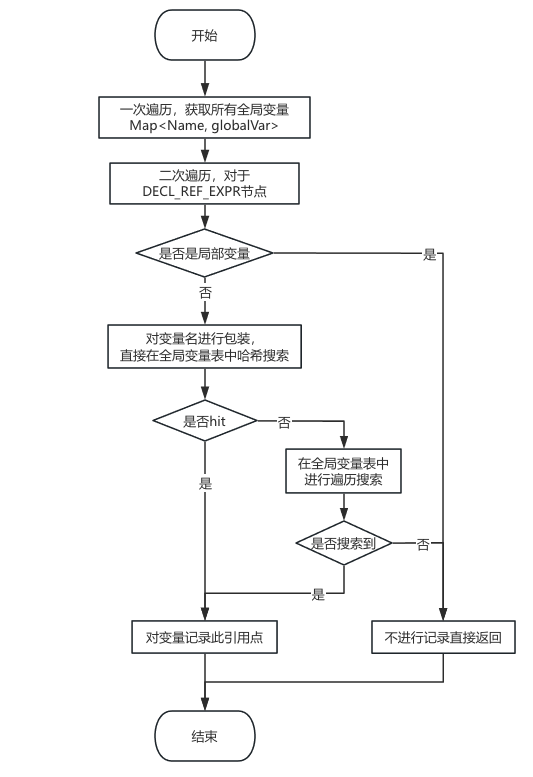
\includegraphics[width = 0.7\textwidth]{全局变量提取流程图.jpg}
\caption{全局变量提取流程图}
\end{figure}

第一次遍历获取所有的全局定义。首先提取所有的
Var\_Decl 节点,它表示变量定义,然后提取节点中的变量名和变量类型。注
意,由于在 AST 中的节点标签中无法区分变量是否是全局的,所以这里根据节点在 AST
中的深度来判断是否是全局变量,并且在变量名前加上针对该项目文件的绝对路径,来
保证变量名的唯一性。在确定其为全局变量后,还需进一步提取该变量的作用域。在
C/C++语言中,static关键字可用于修饰变量和方法,意味着该变量或该方法只能在其所在文
件内使用,而不是全局可用,因此需要对其作用域进行判断。一次遍历提取到的结果是
一个全局变量表,这里使用哈希表 Map<Name, globalVar>的数据结构进行存储,方便对
全局变量进行查找。

第二次遍历的主要目的是提取全局变量的引用点。在方法节点子树中搜索
Devl\_Ref\_Expr 节点,该类型节点表示对变量的引用,这里首先判断被引用的变量是否是局部
变量,根据方法摘要表中该方法的相关信息可以判断,如果是则直接返回,因为我们不关心方法内的局部变量引用。如果不是,则证
明使用的是全局变量,首先在哈希表中进行查找该变量名,以节省检索时长,如果查找到了,说明
是在该文件中定义的全局变量,同时能够保证被 static 修饰的全局变
量的判断的准确性。如果没有查找到,则说明引用了别的文件中定义的全局方法,则在哈希
表中进行遍历查找,记录该全局变量被引用的方法。具体提取流程如图 2-3 所示。

分析结束后,将全局变量的信息组织为全局变量信息表,表的每一项表示一个全局变量的信息,每条信息由\textless \textit{globalVarID}, \textit{type}, \textit{use}, \textit{scope}, \textit{file}  \textgreater 共5部分组成,分别表示全局变量的唯一ID标识,变量类型,变量的引用点所在的方法,变量的作用域以及变量所在模块。



\section{基于依赖关系的变更影响分析}

依赖关系传递闭包方法是一种基于静态依赖关系的技术手段,通过识别代码模块间的关联性划定受变更影响的范围\cite{2021Improving}。其核心思想是利用依赖关系的传递性,通过构建和分析依赖图,揭示所有可能受到影响的代码模块或单元。

\paragraph{构建依赖图}

以抽象语法树、全局变量信息表和方法摘要表为基础,构建程序的系统依赖图。图节点代表代码中的基本元素,本文中是方法和全局变量,而边则表示这些元素之间的依赖关系。依赖关系包括方法调用和全局变量变量引用,在全局变量信息表和方法摘要表中可直接提取依赖关系。生成边的原则如下:
\begin{itemize}
    \item 调用边(call):方法间的调用关系。如果方法A调用了方法B,在图中增加一条从节点A指向节点B的有向边。
    
    \item 引用边(use):方法和全局变量的引用关系。如果方法A引用的全局变量C,在图中增加一条从节点A指向节点C的有向边。
\end{itemize}

通过这种方式,依赖关系图不仅能够系统地表示代码中各个元素之间的直接依赖关系,还能为后续的变更影响分析提供结构化的图形模型。如图2-4为依赖图示例,该图中共有6个方法和3个全局变量,其静态依赖关系如图中的边所示。

\begin{figure}[h]
    \centering
    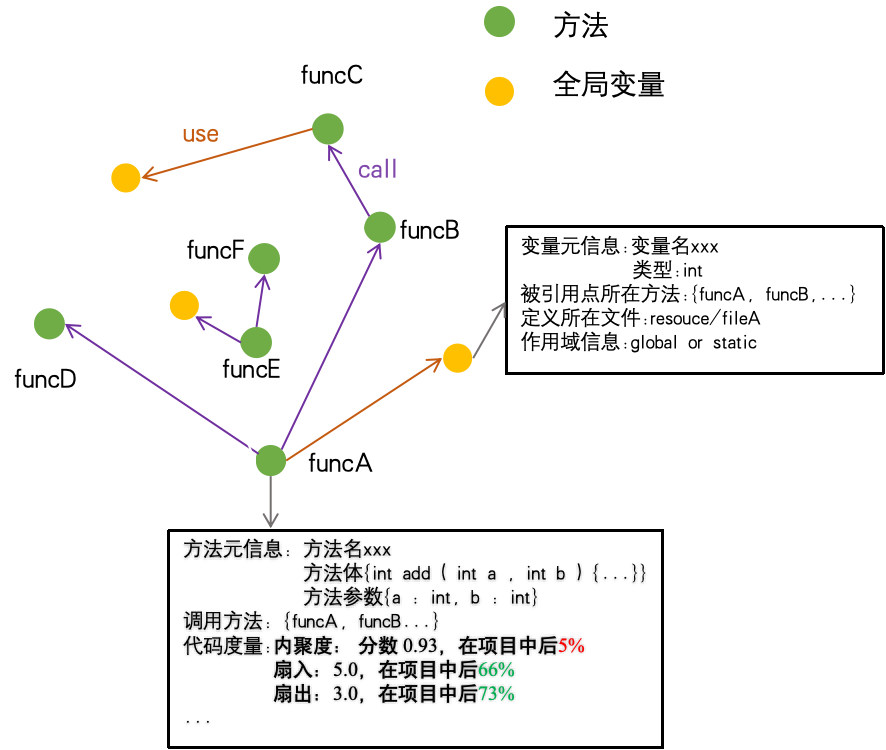
\includegraphics[width = 0.6\textwidth]{依赖关系示例.png}
    \caption{依赖图示例}
    \end{figure}

\paragraph{执行变更影响分析}

这一过程旨在确定哪些方法在代码变更时可能受到影响,以及这些影响的传播路径。本文基于方法和方法之间的以下两种关系RBM(relationships between methods)对每一个方法识别当其变更时受影响的方法集IMS(impacted method set),定义如式(2-1)所示,以方法f和方法g的关系为例,CALL方法和RETURN分别代表f和g的调用和被调用关系。
\begin{equation}
\begin{array}{l}
R B M=C A L L \cup R E T U R N \text { where } \\
(f, g) \in C A L L \Longleftrightarrow f(\text { transitively)calls } g, \\
(f, g) \in R E T U R N \Longleftrightarrow f(\text { transitively)returns into } g
\end{array}
\end{equation}

对于依赖关系图中的每个节点,计算该节点的传递闭包。传递闭包是指从某个特定节点出发,根据上文定义的依赖关系和图的可达性,可以直接或间接到达的所有节点的集合,反映了节点之间的依赖链以及影响传播的范围。传递闭包的具体迭代模型如式2-2。

\begin{equation}
\begin{array}{l}
I M S^{(N)}=I M S_{C A L L}^{(N)} \cup I M S_{R E T U R N}^{(N)} \\
I M S_{ {RETURN }}^{(N+1)}=\bigcup_{define \in (I M S_{R E T U R N}^{(N)}-I M S_{R E T U R N}^{(N-1)} ) } I M S({ define }) \\
I M S_{C A L L}^{(N+1)}=\bigcup_{ {define } \in (I M S_{C A L L}^{(N)})} I M S( { define }){, define } \in \\
\left(I M S_{C A L L}^{(N)}-I M S_{C A L L}^{(N-1)}\right) 
\end{array}
\end{equation}


其中N表示第N轮迭代,第N+1轮的迭代受N和N-1轮的影响,反映出软件系统中的变更的涟漪效应。为了高效地计算传递闭包,使用广度优先搜索遍历图中的各个节点及其依赖边,进而识别出所有直接或间接依赖于某个节点的其他节点。每次从某个节点出发时,都会跟踪并记录通过依赖关系可到达的所有节点,,最终得到的节点集合中,所有的节点都与初始变更的节点存在某种直接或间接的依赖关系。这些方法可以视为受变更影响的范围,意味着它们在该方法变更后,可能会因为依赖关系的传递而受到影响。通过这一分析,我们不仅可以识别出受影响的直接方法,还能揭示出那些通过多次间接依赖而受到影响的方法,帮助开发者全面了解变更的潜在影响范围。


在图 2-1 的例子中,方法 funcA 调用了 funcB 和funcD,funcB 调用了 funcC。在对 funcB 进行变更影响分析时,会直接影响到 funcA和funcC,根据依赖关系闭包,会间接影响到funcD。所以与 funcB 有变更影响关系的方法集合为\{funcA, funcC, funcD\} 。


\section{基于克隆关系的变更影响分析}
代码克隆(Code Clone)是指在代码中存在两段或多段内容相似或完全相同的代码片段。因此它们在逻辑上往往具有相同的功能或行为。如果对其中一个克隆片段进行了变更(例如修复了一个 bug、添加功能或进行优化),那么在其他地方相同或相似的代码也可能需要同步修改,否则可能会导致系统的不一致性或错误,这是典型的逻辑型变更影响关系。

因此,本文基于方法间的克隆关系进行变更影响分析。该方法主要分为两步,首先对源程序进行预处理,通过代码分段及代码指纹提取的方式对源程序进行编码,生成代码序列数据库。随后利用频繁模式挖掘算法ClaSP得到克隆代码列表,具体的处理流程如图3-2所示。

\begin{figure}[h]
\centering
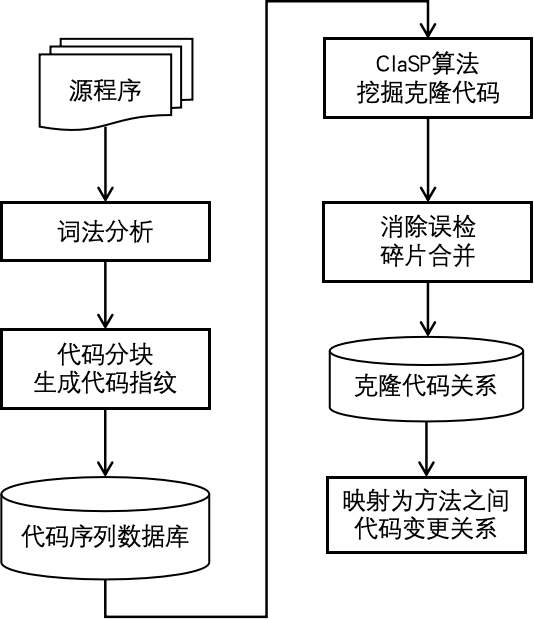
\includegraphics[width = 0.4\textwidth]{代码克隆流程}
\caption{基于代码克隆的变更影响分析方法流程}
\end{figure}

\subsection{代码预处理}

\paragraph{词法分析}

\begin{itemize}
    \item 去除注释:注释通常用于解释代码的意图,并不直接影响程序的执行,但不同的代码实现中注释内容可能存在差异,这会导致本质相同的代码片段由于注释的不同而被误判为非克隆。
    
    \item 去除头文件引用语句:源代码文件往往包含多个头文件,而不同的源文件可能引用相同的头文件。如果不对头文件进行统一的处理,算法就可能在不同的源文件中检测头文件引用的代码克隆情况,可能影响克隆检测的效率和准确性。
    
    \item 程序标准化:为了避免因变量名的变化导致漏检,在方法内部对变量名进行统一标准化处理。

\end{itemize}


\paragraph{代码分块} 这一步将代码拆解成更小、更易于对比的单元,从而提高克隆检测的准确性。本文的代码分块策略按代码结构的不同分为几类,

\begin{itemize}
    \item 顺序结构:按固定行数分块,行数可由用户定义,默认为6行一块。行数越小则识别结果越精准,越能识别更细小的代码克隆情况。
    
    \item 控制结构:将选择结构(if、then、else、endif、switch)、循环结构(while、for)、和域结构(\{、\})共同描述为控制结构识别并根据关键分块词进行分块。这是由于控制语句是代码逻辑的重要分界点,将它们作为分块的标准可以确保检测系统能聚焦于实际功能的逻辑边界。
\end{itemize}

值得注意的是,分块时大括号不被视为代码块的一部分。不同的开发者在代码排版上可能存在差异,例如有的开发者将大括号置于同行,而另一些则习惯将大括号另起一行。为了避免这种格式差异对克隆检测结果产生干扰,大括号被排除在代码块之外。

\paragraph{代码指纹提取} 遍历代码块的每一行语句,将每行语句转化为数字序列,再将所有数字序列合并,转化为代码块的“指纹”。该指纹将代表代码片段用于识别代码片段之间的相似性或重复性。鉴于哈希算法在计算上的高效性与实现的简便性,它在生成代码指纹方面具有显著的优势。因此,本文选择采用冲突率较低的hashpjw算法提取代码指纹。

\subsection{基于代码克隆检测的变更影响关系提取}
序列数据挖掘(Sequence Data Mining,SDM)是时序数据挖掘领域的一个重要研究方向,旨在从给定的输入数据库中,探索在大量对象之间随时间频繁出现的模式。判断一个模式是否具有意义的阈值被称为最小支持度。本文中,将代码指纹片段作为序列,合并起来为序列数据库,利用序列数据挖掘算法,挖掘频繁出现的模式,将问题转化为闭合序列挖掘问题。这里对于数据挖掘的一些基本概念不再赘述,具体可参考文献\cite{2013ClaSP}。

\paragraph{闭合序列挖掘——检测克隆代码片段}主要分为两步,首先生成频繁序列,作为频繁闭合序列的候选FCC(Frequent Closed Candidates)。第二步执行剪枝,从候选中剔除所有非闭合的序列,最终得到精确的FCS(Frequent Closed Set)。主要的算法流程如3-1所示。

\begin{algorithm}
\caption{ClaSP算法}
\KwIn{序列数据库}
\KwOut{频繁闭合序列集 $FCS$}
 $F_1 \gets \{\text{频繁 1-序列}\}$ \\
 $FCC \gets \emptyset$, $FCS \gets \emptyset$  \\
\For{\textnormal{all} $i \in F_1$}
{
    $F_{ie} \gets \{\text{频繁 1-序列的长大于i的扩展序列 } \}$ \\
    $FCC_i \gets \text{DFS-Pruning}(i, F_1, F_{ie})$ \\
    $FCC \gets FCC \cup FCC_i$
}

 $FCS \gets \text{N-ClosedStep}(FCC)$
\end{algorithm}


首先找到所有的频繁的1-序列(即长度为1的序列),然后,对于所有频繁的1序列,递归地探索相应的子树。对所有频率为1的序列进行此处理,得到FCC,最后,算法结束去除FCC中出现的非闭合序列。
    

DFS-Pruning 算法的通过递归生成候选模式(包括 s-扩展和 i-扩展,分别在模式末尾和任意位置添加新元素)并检查其支持度,最终返回以当前模式 $p$ 为前缀的所有频繁模式集。剪枝时,通过检查对应模式的子序列和超序列的支持度,将序列的节点进行合并,防止继续遍历冗余节点。最终得到的FCS即为所有克隆代码集。

\paragraph{合并碎片——提取方法间的变更影响关系}

由于先前的代码分段处理导致克隆代码呈现为片段间的克隆关系,为了恢复代码的完整性,进一步对这些碎片进行合并。基于每段代码的位置信息,将属于同一方法的碎片进行合理整合,从而重建方法间的克隆关系。通过这种方式,最终得到的是方法与方法之间的克隆关系,反映了不同方法之间在代码修改过程中的潜在影响,即方法间的变更影响关系。

\section{基于变更历史和共现关联关系的变更影响分析}

在软件工程中,分析代码变更历史是理解软件演化重要手段之一。在开发者对项目进行维护的过程中,通常是以一个提交(commit)为单位进行功能上的变更。当进入新的维护工作时,如对同一功能进行升级等,通常的做法是参考前人的开发历史,对当前开发工作做指导,以防止变更的不完全。基于这一特点,本文实现了基于变更历史和共现关联关系的变更影响分析方法,分析对象是软件项目的变更历史。该方法能够提取蕴含在代码变更历史中的变更影响关系,尤其适用于具有丰富变更记录的软件项目。

该方法的核心原理是在代码变更历史中,频繁同时更改的代码片段,通常存在着某种潜在的变更影响关系。这种变更影响关系不仅仅局限于静态结构上的依赖,还包括功能上的耦合和实现上的相互作用。因此,通过对这些历史变更数据的深入挖掘和分析,我们可以揭示出更丰富的逻辑型变更关系。

\subsection{代码变更历史提取}

由于 Git 是现代软件开发中最广泛使用的版本控制工具,因此,本文的分析主要基于由 Git 进行版本管理的项目。

\paragraph{收集项目代码库及变更历史记录}克隆项目的代码库到本地,通过git log命令获取所有的commit,包括每个提交的哈希值commitHash等信息。

\paragraph{提取每个提交的变更信息} 对每个提交运行git show <commitHash>命令,查看该提交引入的代码变更(即“diff”或差异),这会显示哪些文件被修改、添加或删除,本文主要关注标记为“修改”的文件,这些修改的文件中包含了具体的代码变化,即代码行的增、删、改操作,记录该commit引起的所有发生变更的代码行。

\paragraph{定位变更代码行所属的方法} 定位变化代码行所在的方法。通过libclang分析变化前文件得到的抽象语法树可获取每个方法对应的代码行,与变更的代码行位置进行匹配,得到变更的代码行所在的方法。

\paragraph{提取变更方法与提交的关系} 对于每个提交,提取出所有受影响的方法(即发生变化的方法),并将这些方法构成一个变更方法列表,用Map<commitID, List<Methods>>的结构存储每个commit变更的方法,作为序列数据库,便于后续分析与处理。


\subsection{基于共现关联挖掘的变更影响关系提取}

基于关联规则(Association Rules)的数据挖掘方法是反映事物之间相互依存性和关联性的一个重要数据挖掘技术,旨在从大量数据中挖掘出有价值的项之间的相关关系。共现关系可以视为关联规则的一种表现形式,它描述了在给定集合中,某一组项(或特征)经常出现在同一事务中。例如,在零售分析中,常见的共现关系是“购买了面包的顾客通常也会购买牛奶”。在这种情况下,“面包”和“牛奶”是一对共现项。

在本文的代码变更影响分析中,共现关系描述的是在一次提交中,哪些方法经常同时发生变更。如果两个方法在多个提交中频繁一起变动,则它们之间可能存在某种依赖关系或变更影响关系。

常用的频繁项集的评估标准有支持度和置信度。支持度表示共现项在数据集中出现的次数占总数据集的比重,用于衡量一组项在数据集中的普遍程度。在代码变更分析中,支持度表示某一方法对在多个提交中同时出现的频率,计算公式如3-3.

\begin{equation}
Support(funcA,funcB)=\frac{num(AB\text{共现})}{num(AllCommits)}
\end{equation}

置信度表示共现项中一个出现后,另一个项出现的概率。变更分析中,置信度度量表示当方法A被修改时,方法B被修改的概率,计算公式如3-4。

\begin{equation}
Confidence(funcA\Leftarrow funcB)=\frac{P(AB\text{共现})}{P(B\text{出现})}
\end{equation}

在前文提取的序列数据库中,进行如下算法3-3的计算。



\begin{algorithm}
    \caption{变更影响方法对挖掘算法}
    \KwIn{序列数据库 $D$, 支持度阈值 $min\_sup$, 置信度阈值 $min\_conf$}
    \KwOut{变更影响方法对 $change\_impact\_pairs$}
     $F_1 \gets \emptyset$  \# 频繁1项集\\  
    \For{all $f \in D$} {
        \If{support$(f) \geq min\_sup$} {
            $F_1 \gets F_1 \cup f$
        }
    } 
    $F_2 \gets \emptyset$  \# 频繁2项集\\ 
    \For{all $(f_1, f_2) \in P = \{ (f_i, f_j) \mid f_i, f_j \in F_1, i \neq j \}$} {
        \If{$\text{Support}(f_1, f_2) \geq min\_sup$} {
            $F_2 \gets F_2 \cup (f_1, f_2)$
        }
    }
    
    $change\_impact\_pairs \gets \emptyset$ \\ 
    \For{all  $(f_1, f_2) \in F_2$} {
        \If{confidence$(f_1, f_2) \geq min\_conf$} {
            $change\_impact\_pairs \gets change\_impact\_pairs \cup (f_1, f_2)$
        }
    }
    \Return{$change\_impact\_pairs$}
    \end{algorithm}

计算得到的即为那些频繁同时变更的方法对,表明它们在变更过程中有着较为显著的相互依赖关系,反映了方法间的变更影响关系。

\section{基于深度学习的变更影响分析}
\subsection{研究动机}

前文中所述的方法均有一定的局限性。

\begin{itemize}

    \item 冷启动问题:当项目代码拥有丰富的变更历史时,可以通过前文中介绍的数据挖掘方法,提取具有变更影响关系的方法对,然而并不是所有软件项目都有变更历史可供我们分析。

    \item 影响类型覆盖不全:在仅有项目源代码的情况下,数据挖掘方法无法直接应用,只使用基于依赖闭包和基于克隆代码的方法,则无法识别除这两种关系外的逻辑型变更影响。
    
    \item 影响模式难以迁移:数据挖掘方法仅能得到变更过的影响关系,对于未变更的方法,无法将相同的影响模式进行迁移。
    
\end{itemize}

因此本文提出基于深度学习的变更影响分析方法,通过训练深度学习模型来进行变更影响关系的预测,从而解决上述问题。

\subsection{数据集来源和数据清洗}

\paragraph{数据集来源}

为了保证深度学习方法能够识别依赖型和逻辑型两种影响关系,我们以数据挖掘方法得到的影响关系作为数据集训练深度学习模型。

将数据挖掘方法的置信度设为1,支持度设为2在示例项目中进行检测,检测到有变更影响关系的方法对作为数据集的正例。为了构建平衡的数据集,通过对项目中的方法进行随机采样,从中选取一些不具有变更影响关系的方法对,作为数据集的负例。

\paragraph{数据清洗}

置信度为1表示方法严格共现,但是支持度为2并不是十分严格的挖掘标准,因此数据集中会存在一些由于偶然共现导致的误报现象。为了排除此种样例,本文结合大语言模型对数据集进行清洗。

大语言模型拥有较强的代码语义理解能力,能够对真实的变更影响关系进行精准识别。通过提示变更影响关系的类型以及对应的含义,能够帮助大语言模型对方法间的影响关系进行推理,从而排除掉误报样例。


\begin{promptbox}{数据清洗推理prompt}

你是一个优秀的代码变更影响关系检测师,能够根据用户给定的方法代码对,判断二者之间是否有变更影响关系。方法间的代码变更影响关系指的是一个方法变化(包括签名或内部逻辑的变化),导致其他方法需要随之更改的现象。

方法之间的变更影响主要分为两类,一类是静态依赖型的,表现为方法间的调用或间接调用关系。另一类则是逻辑型的,表现为方法的实现逻辑或所操作的数据之间存在某种隐含的关联,如共同维护某个数据的一致性、共享某些资源,或功能逻辑有某种预期联系等。

请你对用户给定的一对方法进行判断,判断二者之间是否有变更影响关系。

下面为用户问询的一对方法,

方法1:
...

方法2:
...

请给出你的判断,如果有则回答1,没有则回答0,不需要给出解释。
  
\end{promptbox}



\subsection{基于代码预训练模型的变更影响关系预测}

基于深度学习的影响关系预测任务的输入为两个方法体,输出为两个方法之间存在变更影响关系的概率,概率越接近 1,表明这两个方法之间有关系的可能性越大。

考虑到代码理解的复杂性与深度,本文采用了基于预训练模型的代码表示学习方法,选择了 CodeBERT 作为编码器提取代码的表示。CodeBERT 是一种专为程序代码设计的预训练语言模型,通过大规模的代码语料库预训练,能够学习到代码中的丰富语法结构和语义信息。经过 CodeBERT 模型的表示学习,所得到的向量不仅包含了每个方法体的语法特征,还能够编码代码中的语义关系及其他潜在的编程特征。模型架构如图3-3所示。

\begin{figure}[h]
\centering
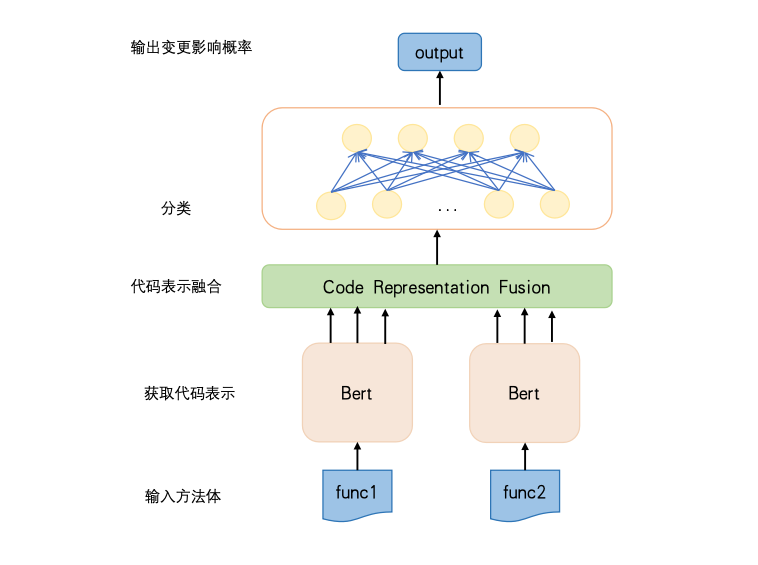
\includegraphics[width = 0.8\textwidth]{模型架构3.jpg}
\caption{基于代码预训练的深度学习模型架构}
\end{figure}


首先,将两个方法体$ F_a, F_b$,先通过代码预训练模型进行编码

\begin{align}
H_a=&Encoder(F_a) \in \mathbb{R}^{(len,dim)} \\
E_a=&mean(H_a[1:...]) \in \mathbb{R}^{(dim)}
\end{align}

得到方法的向量化表示$ E_a, E_b$,通过拼接融合这两个向量,将融合后的向量表示送入一个由两层组成的多层感知机(Multilayer Perceptron,MLP)中,再通过 softmax 层进行分类处理,将模型的输出转化为一个概率分布,表示两个方法体之间存在关系的概率。

\begin{align}
E_{a,b}=Concat(E_a,E_b)& \in \mathbb{R}^{(dim*2)} \\
logits_{a,b}=MLP(E_{a,b})&=FFN(ReLU(FFN(E_{a,b}))) \\
FFN(x)&=Wx+b\\
ReLu(x)&=max(0,x)\\
logits_{a,b}& \in \mathbb{R}^{(2)}
\end{align}

最后与真实标签计算交叉熵损失,得到loss,计算梯度,优化模型参数
\begin{align}
loss=CrossEntryLoss(logits_{a,b}, Label)
\end{align}


\section{实验结果与分析}

\subsection{实验数据与评价方式}

\paragraph{实验数据}

本文从影响力或社区活跃程度的角度出发,收集了表2-2中所示的软件项目为被测项目进行实验。这些项目在github上的收藏数均在千以上,说明这些项目在开源社区中有着一定的影响力,使用范围比较广泛。除antiword项目之外,其他项目有着比较活跃的社区,说明其还在不断更新迭代过程中,所以能提供较为丰富的变更历史,以供数据挖掘方法的实验分析。

\begin{table}[htbp]
\caption{被测项目}
\vspace{0.5em}\centering\wuhao
\begin{tabular}{cp{6cm}ccc}
\toprule
项目名称 & 项目简介 & 代码行数& 提交数 & 收藏数 \\
\midrule
TheAlgorithms & 各种算法的开源实现,涵盖了计算机科学、数学和统计学等领域 & 24645 & 1536 & 57k \\
antiword-0.37 & 提取 Microsoft Word 文档内容的工具 & 34725& - & 13k\\
jemalloc-5.3.0 & 通用的malloc(3)实现,强调碎片避免和可扩展的并发支
持  &83525& 3530 & 9k \\
libbpf-1.1 & linux 内核观测技术的一个脚手架库 & 127927 & 2375 & 1.9k \\
librdkafka-2.1.0& Apache Kafka 的 C/C++ 客户端库 & 154951 & 4430 & 18k \\
FFmpegKit-5.1.0 & FFmpeg 工具包 & 450998 & 369 & 3.7k \\

\bottomrule
\end{tabular}
\end{table}


根据每个示例项目的上一个版本和示例版本间的版本变更,分别各自选取30个变更方法,通过分析commit得到真实的被影响方法集AIS(Actual Impact Set),作为测试集,这里分别统计了依赖型和逻辑型的变更影响关系,得到的数据如表2-3所示。再分别通过前述方法进行检测,得到估计的被影响方法集EIS(Estimated Impact Set),通过评价指标评估方法的有效性。

\begin{table}[htbp]
\caption{被测项目数据统计}
\vspace{0.5em}\centering\wuhao
\begin{tabular}{cccccc}
\toprule
项目名称 & commit数 & 变更点数 & 依赖型AIS & 逻辑型AIS & 总计 \\
\midrule
TheAlgorithms &  & 30 & 98 & 21 & 119\\
antiword-0.37 & - & 30 & 119 & 54 & 173 \\
jemalloc-5.3.0 &   & 30 & 67 & 14 & 81 \\
libbpf-1.1 &  & 30 & 194 & 17 & 211 \\
librdkafka-2.1.0 &  & 30 & 92 & 26 & 118\\
FFmpegKit-5.1.0 &  & 30 & 105 & 17 & 122\\
总计 &  & 180 & 675 & 149 & 824 \\
\bottomrule
\end{tabular}
\end{table}


基于深度学习的变更影响分析方法的数据集收集方式如3.5.1节所述,为了保证测试集和训练集的不重叠性,在经过挖掘和清洗后得到的关系中排除上述测试变更点。得到的数据集统计信息如表3-2所示,共7351对数据,按照训练、验证、测试集 为 6:2:2 进行训练和测试。这里排除了antiword项目,因为该项目并没有官方维护的github仓库,因此无法获得足够的历史变更。

\begin{table}[htbp]
\caption{数据集统计信息}
\vspace{0.5em}\centering\wuhao
\begin{tabular}{cccc}
\toprule
项目名称 & 正例对数 & 负例对数 & 总对数 \\
\midrule
TheAlgorithms & 97 & 1000 & 1097 \\
jemalloc-5.3.0 & 593 & 1000 & 1593 \\
libbpf-1.1 & 401 & 1000 & 1401 \\
librdkafka-2.1.0 & 932  & 1000 & 1932 \\
FFmpegKit-5.1.0 & 103 & 1000 & 1103 \\ 
总计 & 2126 & 5000 & 7126 \\
\bottomrule
\end{tabular}
\end{table}

\paragraph{评价指标}

评价指标如式(3-13)(3-14)(3-15)所示,真实的被影响方法表示为AIS(Actual Impact Set),每种方法检测得到的结果为估计的被影响方法EIS(Estimated Impact Set),按逻辑型和依赖型对关系进行划分,根据这两个值计算精确度、召回率和F-measure,这三种评价指标在信息检索的场景下被广泛使用,本章中用于评价变更影响分析方法的有效性。
\begin{equation}
{precision} = \frac{|EIS \cap AIS|}{|EIS|}
\end{equation}

\begin{equation}
{recall} = \frac{|EIS \cap AIS|}{|AIS|}
\end{equation}

\begin{equation}
F-measure = \frac{2 \times precision \times recall}{precision + recall}
\end{equation}

\subsection{实验设置与实验过程}

\paragraph{实验设置}

\begin{itemize}
    \item 代码预训练模型选择:本文使用了CodeBERTa-small-v1和codebert-base-mlm两个模型分别作为代码表示学习模型,得到的代码表示为768维,融合时使用的MLP的每层维数为(768*2,64,2)。根据在数据集上的表现,选择表现较好的模型与其他方法做对比。
    
    \item 深度学习模型参数设置模型的参数设置如表3-3。

    \begin{table}[htbp]
    \caption{模型参数设置}
    \vspace{0.5em}\centering\wuhao
    \begin{tabular}{cc}
    \toprule
    超参数 & 数值  \\
    \midrule
    Token embedding size & 768 \\
    codeBERT learning-rate  & 1e-5 \\
    codeBERT dropout & 0.4 \\
    Classifier learning-rate& 1e-4 \\ 
    Adam $\beta_1$  & 0.95  \\
    Adam $\beta_2$ & 0.999  \\
    batch\_size & 64 \\
    \bottomrule
    \end{tabular}
    \end{table}   

    \item 基于共现关系方法置信度:设为1。

    \item 基于共现关系方法支持度:设为2和3分别进行实验,选择表现较好的与其他方法做对比。
    
\end{itemize}


\paragraph{实验过程}

    
    基于深度学习的方法在数据集上的实验结果如表3-5所示,从总体上来看,两个模型的性能均表现出色,但模型CodeBERTa-small-v1的F-measure略高于codebert-base-mlm,该模型更强调预测出的正例的真实性和准确性。这意味着它在确保预测结果的准确性方面做得很好。由于其良好的综合能力,选择CodeBERTa-small-v1模型作为主模型进行对比实验。
    
    \begin{table}[htbp]
    \caption{基于代码预训练模型的变更影响关系在数据集上的实验结果}
    \vspace{0.5em}\centering\wuhao
    \begin{tabular}{cccc}
    \toprule
    模型& F-measure & recall & precision \\
    \midrule
    CodeBERTa-small-v1 & 91.8 & 86.1 & 98.2 \\
    codebert-base-mlm  & 87.1 & 100.0  & 77.1 \\
    \bottomrule
    \end{tabular}
    \end{table}

\subsection{实验结果与对比分析}

本节将通过实验对比来评估本章中提出的基于深度学习的变更影响分析方法的性能,这里主要讨论下列三个问题:

RQ1:本章提出的基于深度学习的方法能否有效检测变更影响关系?与其他方法相比,它在精确率,召回率和F-measure上表现如何?

RQ2:四种方法在提取依赖型(DB)和逻辑型(LB)的变更影响关系上各自的优势如何?尤其是对于逻辑型的影响关系是否具有实际意义?分别适用于哪些特殊场景?又各自有怎样的局限性?


\textbf{1.针对于RQ1的实验}

三种方法的实验结果如表3-4所示。


整体上讲,基于深度学习的方法表现最好,其F-measure在所有方法中表现最优,并且在查全和查准的能力上较为平衡。这说明基于深度学习的方法能够学习到过去变更历史中的行为模式,并能将学习到的变更关系知识进行迁移,用于判断新的影响关系。

其次基于共现关系的方法也较为良好。这表明,代码变更历史中方法的共现关系的确蕴含了大量能够有效揭示变更影响关系的信息。这是因为变更历史中都是前人对软件项目进行变更的记录,这样的提交由开发者精确变更,并经历过开源项目中非常严格的审查过程才合入主分支,因此较为准确地反映了代码变更中的实际操作,从而也能将过去的开发模式反映在数据挖掘的结果集中。

\begin{table}[htbp]
\caption{变更影响实验结果 - F-measure/召回率/精确度}
\vspace{0.5em}\centering\wuhao
\begin{tabular}{cccccccc}
\toprule
方法 & F-measure & recall & precision  \\
\midrule
依赖关系 & 42.2 & 81.3 & 28.5  \\
克隆关系 & 6.4 & 3.3 &  92.0 \\
共现关系 & 62.1 & 68.7 & 56.6 \\
深度学习 & 65.2 & 69.4 & 61.4 \\
\bottomrule
\end{tabular}
\end{table}

而另外两种方法表现则较为失衡。基于依赖关系闭包的方法表现为召回率较高而准确率很低,仅为28.5\%。这是由于依赖闭包方法本身的特性决定的,由于变更影响关系随涟漪扩散效应,越向外扩散影响越小,但该方法却平等地认为扩散所至的代码均存在影响关系,这并不不符合涟漪效应的特性。如在图3-4中所示是antiword项目中从bTranslateImage方法出发得到的部分依赖图,它层层递进地展示了从word中提取jpec图片的过程,bTranslateImage调用bTranslateJPEG,处理jpec图片,再调用vASCII85EncodeFile,将图片提取为文件,再依次调用vASCII85EncodeArray和vASCII85EncodeByte。当对Byte方法进行变更影响分析时,根据RETURN关系的涟漪效应,最终会将图中所示的其他4个方法都列为影响集。然而实际上,该方法只对\{Array, File\}存在变更影响关系,最显然的,当Byte方法的签名发生改变时,将直接影响到\{Array, File\},这两个方法如果不更改将发生编译错误。而对另两种方法的影响则微乎其微,化为了动态运行时内部值的变化。

\begin{figure}[h]
\centering
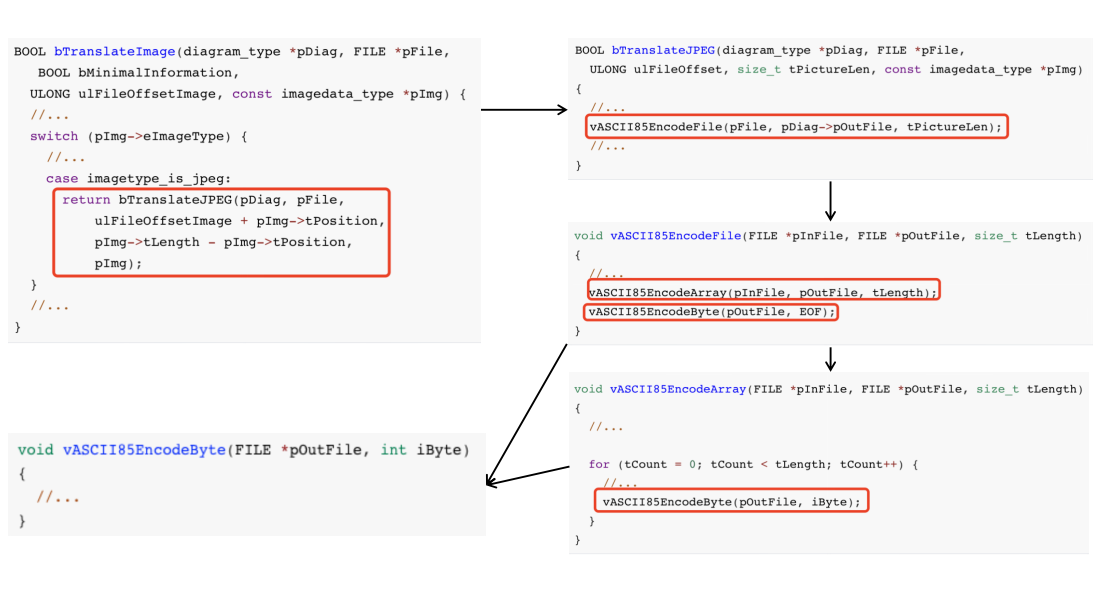
\includegraphics[width = 1\textwidth]{静态分析拒绝样例.jpg}
\caption{依赖闭包方法迭代路径}
\end{figure}

而基于克隆关系的检测方法则更为特殊,其精确率最高,这说明其识别的正例非常准确,很少出现误报。但是它的召回率极低,表明该方法对大部分的变更影响关系无法识别到。这是由于该方法只能识别由于克隆关系产生的变更影响,而在质量良好的项目代码中,克隆代码的现象很少出现,因此提取到样例本身也较少,就导致其整体效果不佳。在实践中,建议基于克隆关系的方法作为其他方法的补充使用。

\textbf{2.针对于RQ2的实验}

RQ1中从整体的角度上说明了三种方法的有效性。为了回答RQ2,这里对每种方法检测得到的依赖型和逻辑型的变更影响关系分别进行计算,得到如表的结果。通过对两种类型分别的统计,我们能更直观地发现不同方法的优势和特点。


\begin{table}[htbp]
\caption{变更影响实验结果 - F-measure/召回率/精确度}
\vspace{0.5em}\centering\wuhao
\begin{tabular}{cccccccc}
\toprule
方法 & DB-F-measure & DB-recall & DB-precision & LB-F-measure & LB-recall & LB-precision  \\
\midrule
依赖闭包 & 44.0 & 96.2 & 28.5 & 0 & 0 & 0 \\
克隆代码 & 0 & 0 &  0 & 31.95 & 19.1 & 97.8 \\
历史共现 & 60.3 & 65.9 & 55.6 & 69.3 & 81.7 & 60.2 \\
深度学习 & 63.0 & 66.3 & 60.1 & 74.4 & 83.4 & 67.2 \\
\bottomrule
\end{tabular}
\end{table}


\paragraph{依赖关系闭包方法}

\begin{itemize}

    \item 优势:对于依赖型影响几乎没有漏报。召回率高达96.2\%,能查全大部分的依赖型影响关系。

    \item 局限性:依赖型影响关系的误报较高,导致依赖型的检测表现整体上较差。针对逻辑型的变更,该方法则无法检测到,这是由于逻辑型的影响关系无法在依赖图中产生联系,因此依赖闭包方法无法检测。
    
\end{itemize}


\paragraph{克隆关系方法}

\begin{itemize}

    \item 优势:逻辑型影响几乎没有误报,其准确率能达到95\%,说明其非常擅长挖掘逻辑型中由于克隆代码导致的变更影响关系。而这种关系在软件长期的维护中容易被忽略。

    图3-6为克隆代码方法挖掘到的一对有变更影响关系的方法。这里展示了这对方法的部分代码,其中绿色高亮的部分表示代码克隆的区域。这两个方法的主要功能是分别对8位和4位压缩格式的图像进行解码。我们发现,这对方法中的大部分逻辑结构几乎完全相同,只有少部分关键处理逻辑存在差异。由此,我们可以认定,这两个方法的变化过程很可能是同步的,即在实际的维护过程中,当对其中一个方法进行修改时,另一个方法也通常需要同步进行相应的变更,才能保证逻辑的一致性。

    \begin{figure}[h]
    \centering
    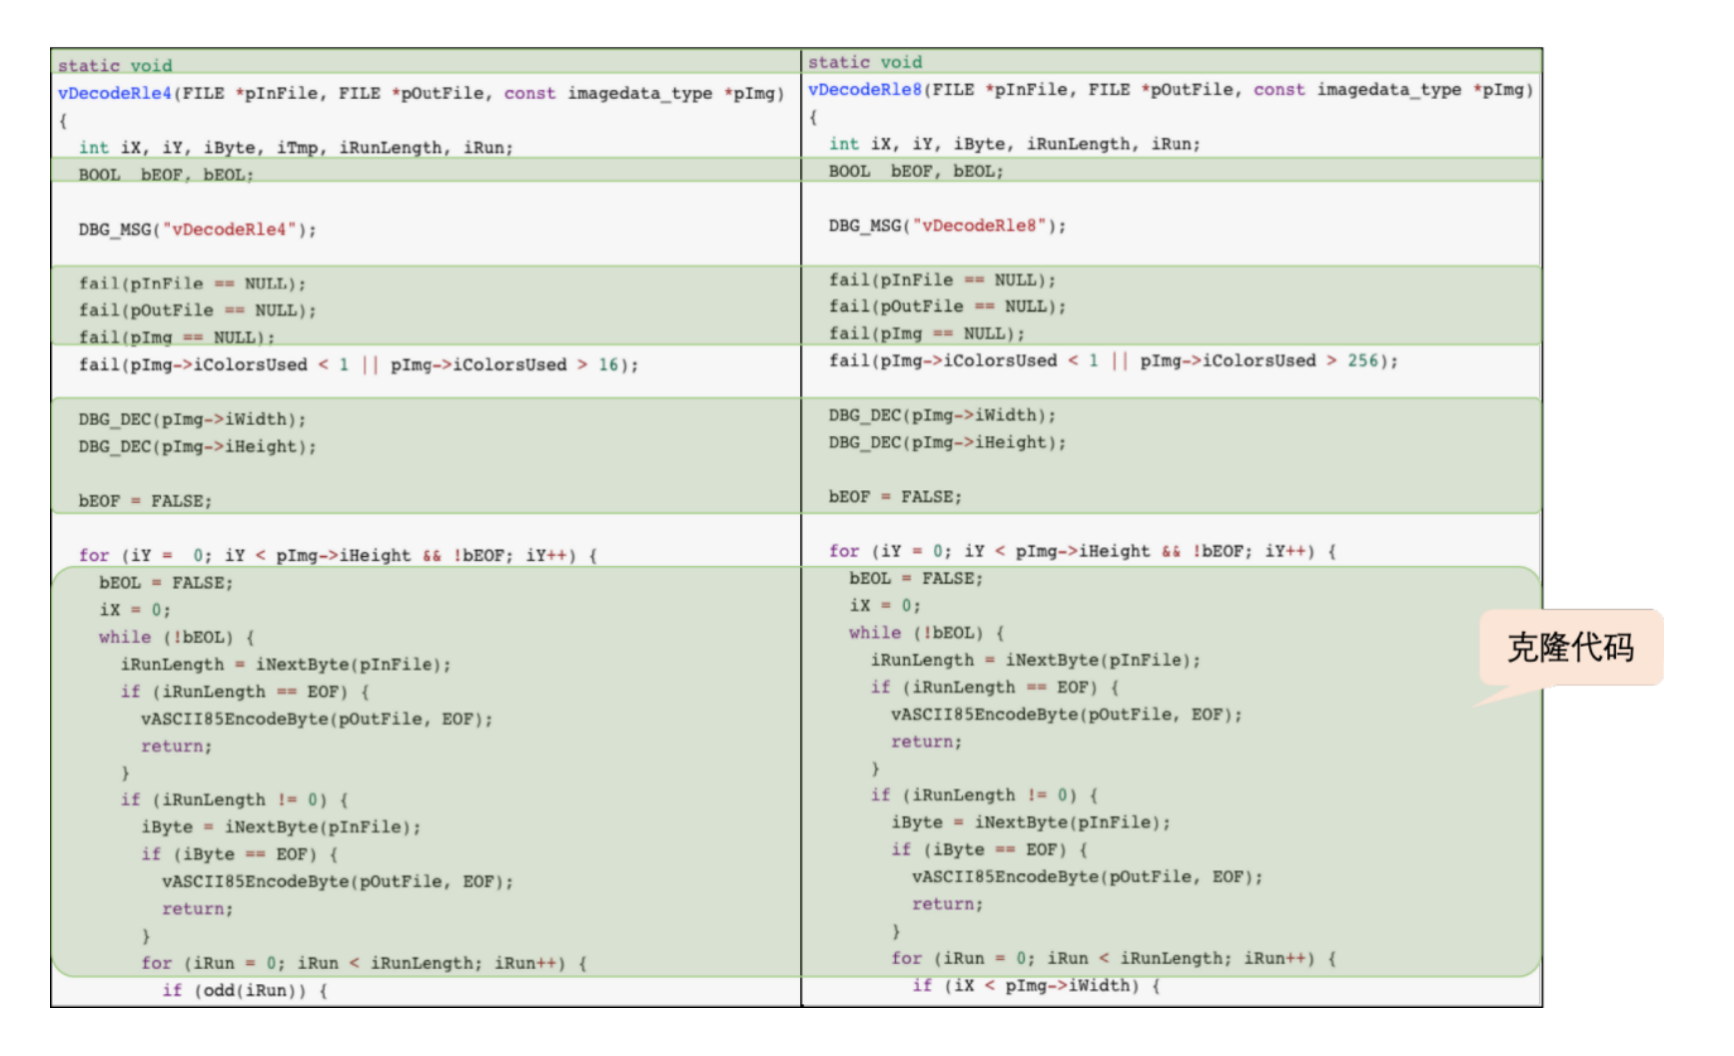
\includegraphics[width = 1\textwidth]{克隆代码示例.jpg}
    \caption{包含克隆代码片段的一组方法实例}
    \end{figure}

    这种现象表明,在软件的演化过程中,维护人员可能需要对这两个方法进行联动更新。任何对其中一个方法的修改都可能影响到另一个方法的功能或逻辑一致性,在代码维护时必须考虑它们之间的相互依赖关系。因此这种基于代码克隆的方法有着非常重要的实际价值。

    \item 局限性:仅能检测检测由于代码克隆导致的逻辑型影响,对于其他逻辑型和依赖型影响存在漏报。
    
\end{itemize}


\paragraph{数据挖掘方法}

\begin{itemize}

    \item 优势:可以挖掘两种类型的变更影响关系。对于依赖型影响,尽管有一定的漏报,但是误报较少,对比依赖闭包方法有着更强的实用价值。而对于逻辑型影响,其表现优于依赖闭包和克隆代码方法,说明其不仅仅只关注了克隆一种关系,还包括其他逻辑型的关系。
    
    以 librdkafka 项目中挖掘到的一对方法为例,该项目是 Apache Kafka 的一个高性能 C/C++ 客户端库。图 3-7 左侧的方法rd\_kafka\_global\_cnt\_decr负责对计数器进行减一操作,而右侧的方法rd\_kafka\_global\_cnt\_incr则负责对计数器进行加一操作。

    \begin{figure}[h]
    \centering
    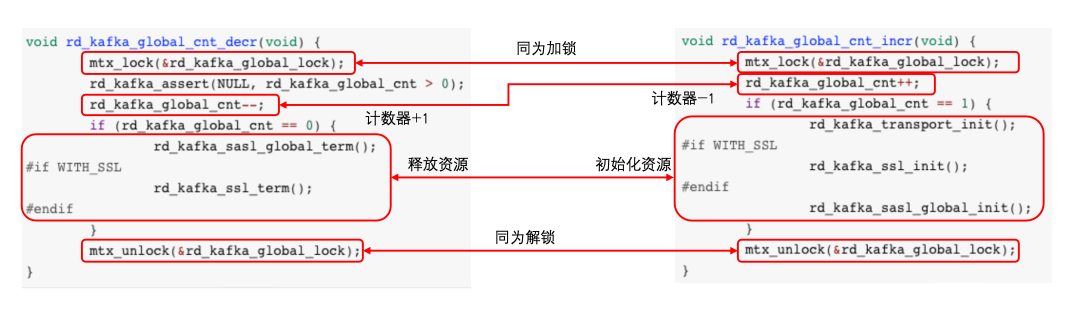
\includegraphics[width = 1\textwidth]{incrdec.jpg}
    \caption{逻辑上有变更影响关系的方法对示例-incr和decr}
    \end{figure}

    从功能上来看,这两个方法是一对典型的协作方法,其作用密切相关。具体来说,incr方法执行计数器加一操作,在计数器从零变为一时,执行资源的初始化工作。而 decr方法则在计数器减为零时,执行资源的释放操作。从代码实现可以看出,这两个方法的操作逻辑具有明显的互补性,加一与减一、初始化与释放的功能关系呈现出“镜像”特性。

    尽管它们依赖图上无法产生联系,但由于它们在功能上承担了计数器的管理和资源的初始化与释放工作,其逻辑关联性非常强。因此,当其中一个方法的实现逻辑发生变化时,另一个方法通常需要进行相应的调整,以保持整体逻辑的一致性,这种方法对的变更影响关系属于典型的逻辑关联型变更影响关系。因此也有较强的实用价值。

    \item 局限性:
    \begin{itemize}
        \item 要求项目代码必须有变更历史。
        \item 挖掘算法的支持度对结果有影响。表是支持度分别为2和3对应的实验结果。可以发现,支持度越大,误报越少,但是漏报越多。这说明支持度越大越排除了一些变更共现的偶然因素,但是失去了对影响关系的普遍性检测,能检测出的关系更少,导致了漏报增加。
        
        \begin{table}[htbp]
            \caption{变更影响实验结果 - F-measure/召回率/精确度}
            \vspace{0.5em}\centering\wuhao
            \begin{tabular}{cccccccc}
            \toprule
            方法 & DB-F-measure & DB-recall & DB-precision & LB-F-measure & LB-recall & LB-precision  \\
            \midrule
            历史共现-2 & 60.3 & 65.9 & 55.6 & 69.3 & 81.7 & 60.2 \\
            历史共现-3 & 63.3 & 54.5 & 75.4 & 76.1 & 69.3 & 84.3 \\
            \bottomrule
            \end{tabular}
            \end{table}

        \item 挖掘到的信息属于硬信息。仅依靠变更历史的只能得到变更过的方法之间影响,未变更过或变更次数较少的影响关系无法反映,相同的影响模式之间无法进行迁移。
        \end{itemize}
    
\end{itemize}



\paragraph{深度学习方法}

\begin{itemize}

    \item 优势:可以挖掘两种类型的变更影响关系且效果较好。解决了没有变更历史的冷启动问题,对于逻辑型影响也能够实现影响模式的迁移。

    \item 局限性:主要体现为计算性能问题。以antiword项目为例,方法共578个,测试变更点有30个,对每个变更点都需与项目所有方法一一计算就是30*(578-1)=17310次,均需要通过嵌入、分类过程。耗费较长的时间,导致实际可用性大打折扣。
    
\end{itemize}
    

上述方法为代码变更影响关系的检测提供了多样化的解决方案,但是各有侧重,适用于不同的应用场景,同时也具有一定的局限性。总结如表3-7。


\begin{table}[htbp]
\caption{变更影响分析方法对比总结}
\vspace{0.5em}\centering\wuhao
\begin{tabular}{ccp{4cm}p{4cm}}
\toprule
方法& 检测关系 & 优势 & 局限性\\
\midrule
依赖闭包 & 依赖型 & 依赖型漏报低 & 依赖型误报高,且仅能检测依赖型\\
克隆代码 & 逻辑型中的代码克隆 & 逻辑型中克隆关系影响的误报低 & 只能检测代码克隆一种关系\\
数据挖掘  & 依赖型和逻辑型 & 两类影响的性能均较好 & 无法应用于没有变更历史的项目,不频繁变更无法被检测 \\
深度学习  & 依赖型和逻辑型 & 两类影响的性能均较好 & 性能问题 \\
\bottomrule
\end{tabular}
\end{table}



\section{本章小结}

本章实现了基于依赖闭包、克隆代码、变更历史共现挖掘的变更影响分析方法,并提出了基于深度学习的影响分析方法。经过实验验证了基于深度学习方法的有效性,并通过分析四种方法在依赖型和逻辑型的表现,总结了四种方法各自的优点和局限性。

% Local Variables:
% TeX-master: "../main"
% TeX-engine: xetex
% End:
